\documentclass[aspectratio=169]{beamer}
\usetheme{Madrid}
\usepackage{booktabs,graphicx}
\title{Compositional Cross-Panel VQA}
\subtitle{Reasoning over compound women's-health figures with frozen embeddings}
\author{Anonymous Authors}
\begin{document}
\frame{\titlepage}
\begin{frame}{The benchmark's revealing exclusion}\centering\Large ``The VLM can't see the whole figure.''\\[1em]\normalsize A single crop cannot compare sibling panels, find an outlier, or count a modality.\end{frame}
\begin{frame}{Compound figure to panel set}\centering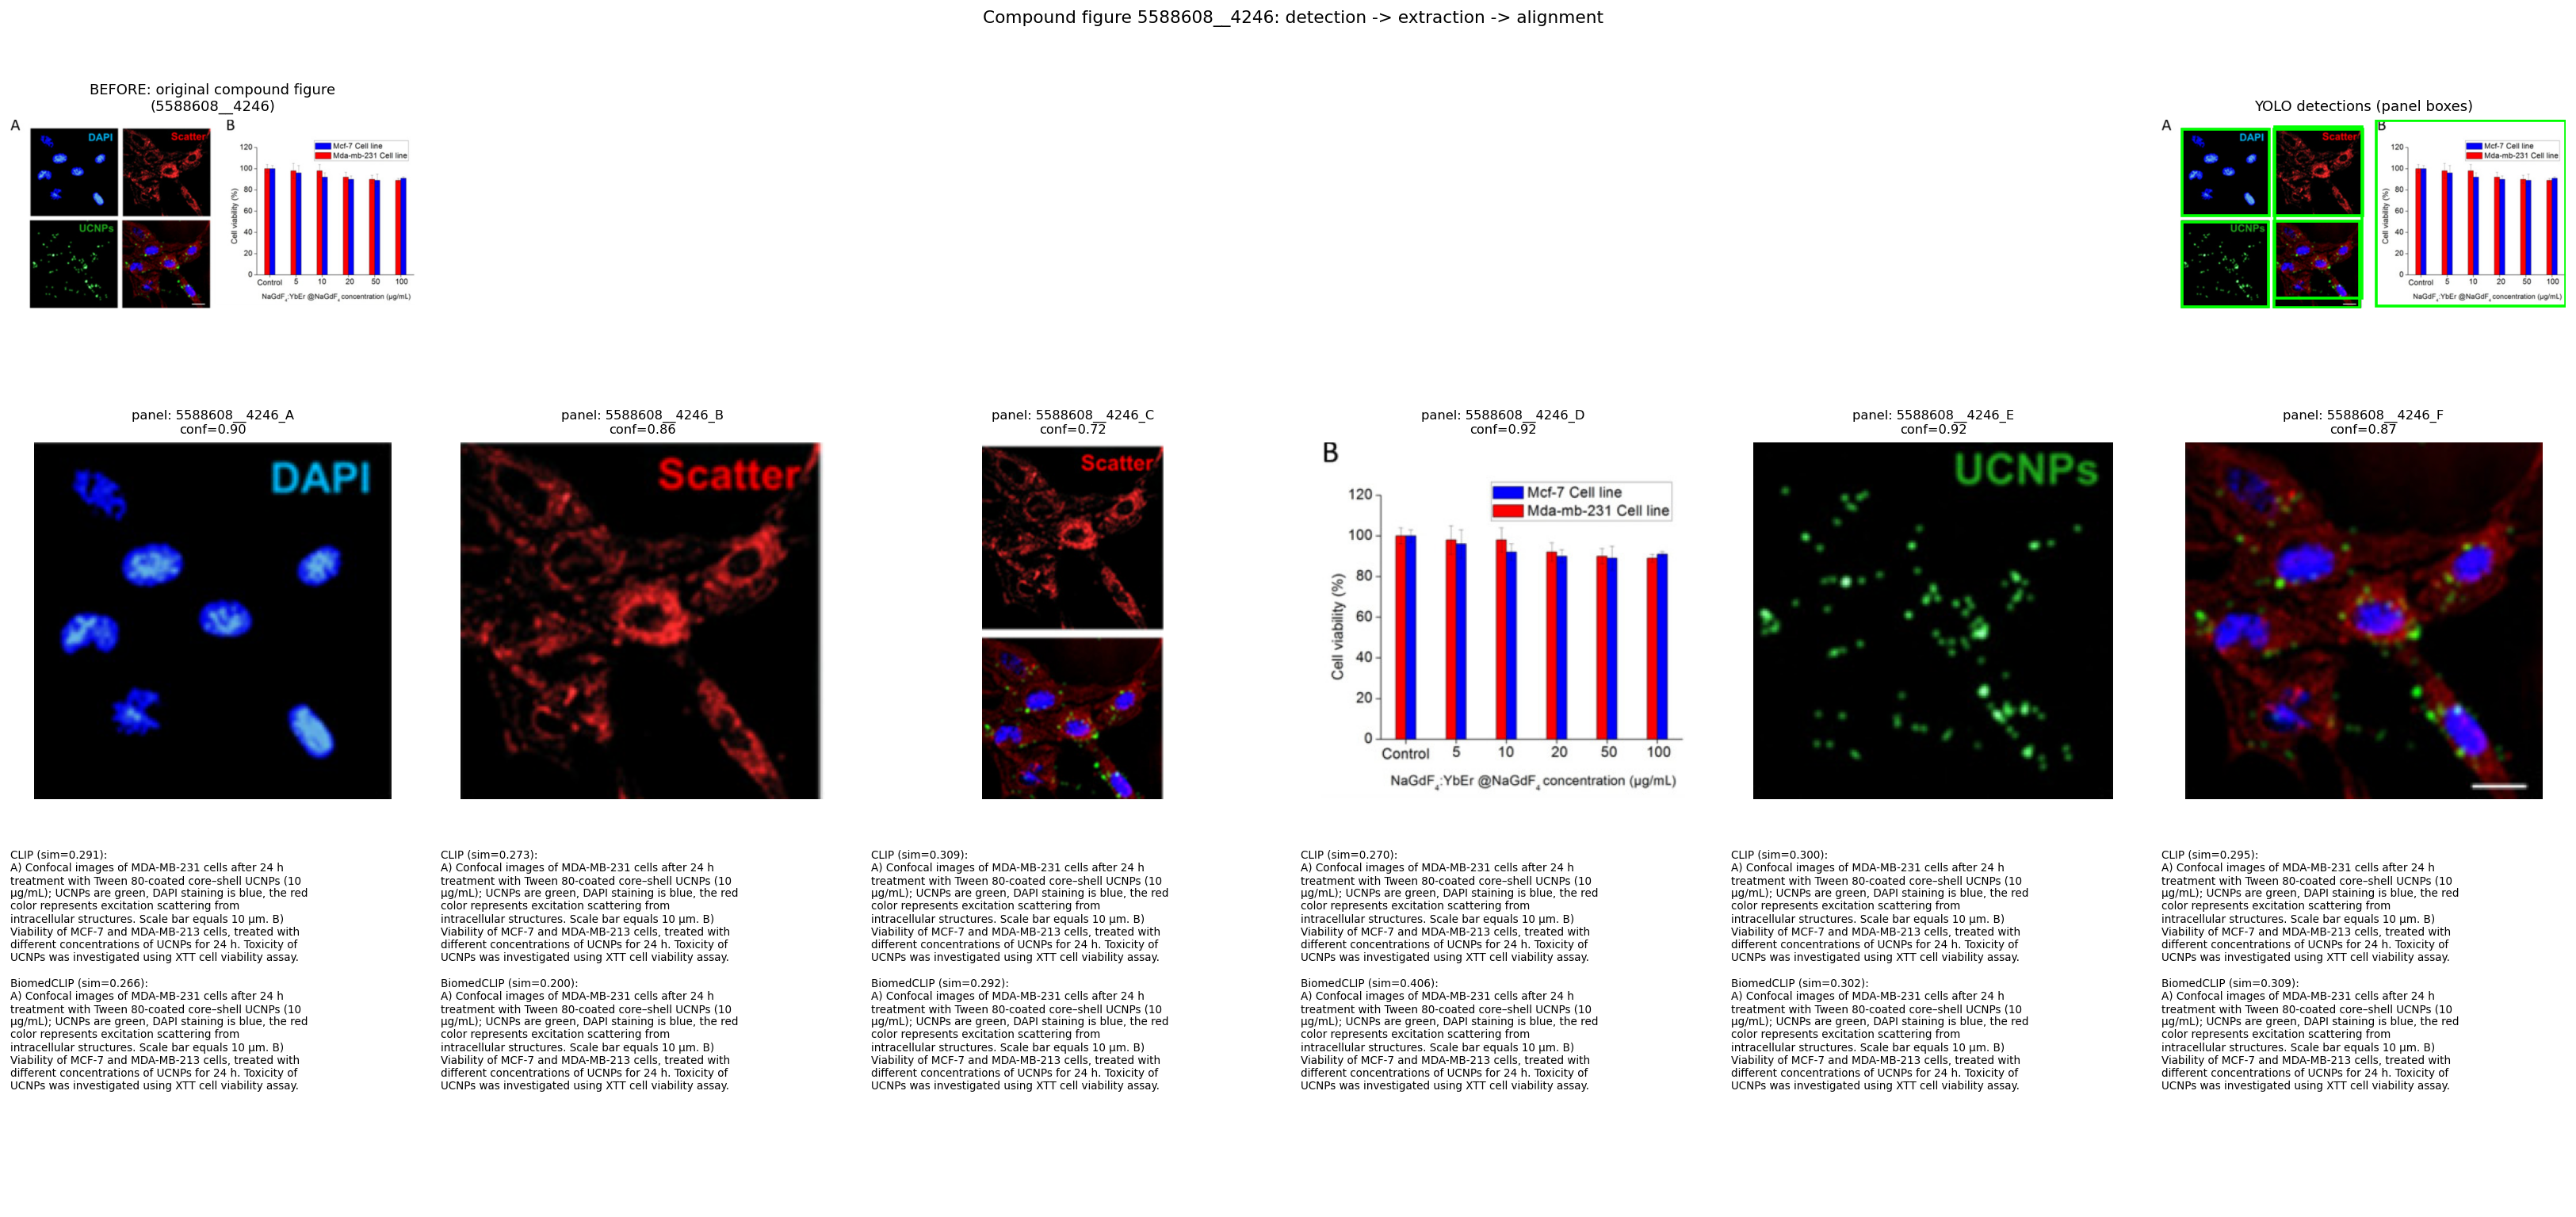
\includegraphics[width=.82\linewidth]{../figures/5588608__4246_demo.png}\\\small Existing detection gives ordered crops; Stage 11 consumes the full accepted set.\end{frame}
\begin{frame}{Contributions}\begin{itemize}\item Categorical, auditable cross-panel VQA task\item One-to-one constrained caption alignment\item Reading-order-aware panel-set attention over frozen embeddings\item No-new-inference baseline from saved per-panel predictions\end{itemize}\end{frame}
\begin{frame}{Three question families}\begin{enumerate}\item Do panels A and B show the same modality?\item Which panel shows a different anatomy?\item How many panels show MRI?\end{enumerate}Only unambiguous categorical answers are generated.\end{frame}
\begin{frame}{Eligibility and leakage safety}\begin{itemize}\item At least three accepted panels\item At least two panels with non-null modality or anatomy tags\item One same and one different pair when available\item Ambiguous anatomy cases skipped\item Paper-level split inherited and asserted per figure\end{itemize}\end{frame}
\begin{frame}{Repairing alignment collapse}\centering Independent argmax $\rightarrow$ Hungarian one-to-one assignment\\[1em]Low similarity $<0.18$ is rejected; unavoidable sharing and unsplit captions are explicitly flagged.\end{frame}
\begin{frame}{Method}\centering Frozen panel embeddings + reading-order embeddings\\$\downarrow$\\multi-head self-attention\\$\downarrow$\\question-conditioned weighted pooling\\$\downarrow$\\question-type classification head\end{frame}
\begin{frame}{What trains?}\begin{itemize}\item Attention, positional embeddings, and small MLP heads only\item CLIP/BiomedCLIP image and text towers remain frozen\item Question strings embedded once and cached\item Seed 42; one fixed configuration\end{itemize}\end{frame}
\begin{frame}{Ablation ladder}\begin{enumerate}\item Saved single-panel VLM tags + deterministic composition\item Mean pooling (no position, no attention)\item Set attention (proposed)\item CLIP vs. BiomedCLIP where caches exist\end{enumerate}\end{frame}
\begin{frame}{Evaluation}\begin{itemize}\item Exact accuracy overall and by question family\item Missing saved panel prediction $\Rightarrow$ exclude, never impute\item Report evaluated/excluded counts and prediction distributions\item No new VLM inference\end{itemize}\end{frame}
\begin{frame}{Results}\IfFileExists{../paper/tables/results_table.tex}{\centering\resizebox{\linewidth}{!}{\begin{tabular}{llrrrrr}
\toprule
Method & Backbone & $n$ & Overall & Same/diff. & Odd-one-out & Count \\
\midrule
blip2-opt-2.7b & biomedclip & 0 & -- & -- & -- & -- \\
paligemma-3b & biomedclip & 0 & -- & -- & -- & -- \\
qwen2-vl-2b & biomedclip & 0 & -- & -- & -- & -- \\
blip2-opt-2.7b & clip & 1 & 100.0 & 100.0 & -- & -- \\
paligemma-3b & clip & 0 & -- & -- & -- & -- \\
qwen2-vl-2b & clip & 1 & 100.0 & 100.0 & -- & -- \\
mean-pool ablation & biomedclip & 164 & 50.6 & 71.2 & 0.0 & 34.4 \\
mean-pool ablation & clip & 103 & 53.4 & 79.2 & 0.0 & 31.5 \\
set-attention (proposed) & biomedclip & 164 & 52.4 & 71.2 & 0.0 & 37.8 \\
set-attention (proposed) & clip & 103 & 50.5 & 77.1 & 0.0 & 27.8 \\
\bottomrule
\end{tabular}}}{\centering\Large Results pending\\[1em]\normalsize Run Stage 11.1--11.6 against real pipeline data.}\end{frame}
\begin{frame}{Reproducibility contract}\begin{itemize}\item Every path configurable via \texttt{PIPELINE\_ROOT}\item Synthetic tests precede real-data execution\item Metrics saved as JSON; paper tables generated by script\item Missing results stay visibly missing\end{itemize}\end{frame}
\begin{frame}{Limitations}\begin{itemize}\item Single seed and one configuration\item Conservative categorical keyword coverage\item Alignment and detector reading order can be wrong\item Baseline subsets differ when saved predictions are missing\item One clinical domain; no free-form clinical synthesis\end{itemize}\end{frame}
\begin{frame}{Takeaway}\centering\Large Cross-panel reasoning is a distinct capability.\\[1em]\normalsize A tiny head over frozen embeddings can test it cheaply and audibly.\end{frame}
\end{document}
